\begin{comment}
	Split data according to percentile
	RFCN resnet-101
	Pascal voc heavily skewed to smaller objects. Show plot
	50th percentile 13892.0
		test data also split according to this value
		cannot simply do by image basis - some images have multiple objects GTs - show figure
			total of 12275 GTs when doing this, still 3384 that are larger
		test images if only small images present - 697 images, 


	Results
		RFCN ResNet-101: 0.7632
		Model - 07++12 < 50th percentile
			All data: 0.5960


    %%%%%%%%%%%%%%%%%%%%%%%%%%%% RFCN 5 Stage Split%%%%%%%%%%%%%%%%%%%%%%%%%
    Train networks with object proposals from an RPN network
        many more object proposals than using GTs - 9,979,342 vs 80,116
            split also different due to this - skew towards smaller objects
                Median of GTs - 19,205.5 vs RPN GTs - 4,864.0
    Objective is to split data into equally size. What is more correct? Equal size based on true GTs or on RPNs
        if based on GT median - Small - 6,410,914 (64.25\%) vs Large - 3,598,428 (35.75\%)
        if based on RPN median - Both - 4,989,671 (50/50)
    However, test may not be equally as split
        Test proposals for network - Total - 1,418,317
            Split on GT - Small - 790,607 (55.74\%) Large -  627,710 (44.25\%)
            Split on RPN - Small - 540,767 (38.0\%) Large - 877,550 (61.87\%)

    RPN GT Training
        RPN proposals is much larger than training with only GTs
            using only GTs 80,116 vs 9,989,342
                due to proposals finding many more examples
            however, still only the correct amount of GTs labels. eg. GT = 3, background = 300
        therefore, when splitting important that one of the splits does not have significantly less GT examples.
        if split by GT median (19,205.5)
            equal number of GT training examples - 40,058 - fits well with GT
            background examples - Small - 3,528,370 vs Large - 6,370,859
        if split by all median
            skew towards larger objects
            Small - 19,992 vs Large - 60,116
            Background  - Small - 4,929,297 vs Large - 4,969,369


\end{comment}




\section{Resolution-Aware Object Detection}\label{sec:resawareSec}
Object detectors are commonly more accurate on objects that cover a larger number of pixels in an image. This is intuitive as objects with a lower resolution objectively have less details that can describe them. The poorer performance can be seen in \tableref{cocores}, for all object detectors the \gls{ap} is considerably lower for smaller objects in comparison to both medium and large. The best performing detector from \cite{deepres}, has an \gls{ap} difference of 35.3\%, from 50.9\% for large objects to 15.6\% for small. 
A potential method of tackling this issue is to train multiple detectors on separate partitions of the training data according to the size of the object. While deep-based \gls{cnn} have millions of parameters to generalise from training to tesitng, the difference between small and large objects may skew the learning towards the latter. In order to test this hypothesis an initial test will be conducted on the \gls{pascalvoc} dataset. However, \gls{pascalvoc} does not have the same definition of objects sizes as in \gls{mscoco}. Therefore, the distribution of the bounding boxes from the training set must be analysed in order to determine an appropriate split of data based on object size. This was done by parsing all of the bounding box coordinates in the 07++12 training set and calculating the area. A histogram of the area can be seen in \figref{0712hist}. There is a clear tendency to smaller objects in the training set with a clear skew towards the left of the figure.

\begin{figure}[H]
  \centering
    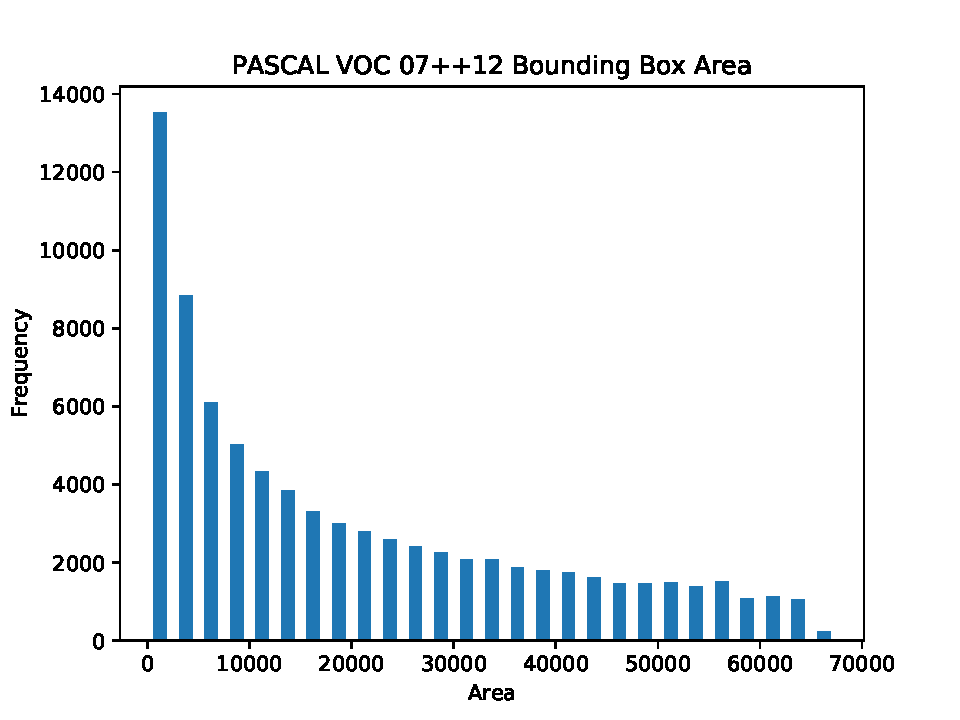
\includegraphics[width=0.6\textwidth]{Figs/Implementation/0712hist.pdf}
      \caption{Histogram of the \gls{pascalvoc} 07++12 bounding box area.}
    \label{fig:0712hist}
\end{figure}

As there is no clear way to split the data into three sets with equal amounts of data, the split was instead done into into two sets, one for small objects and another for larger. The split was made at the median bounding box area which is 13,892 pixels. Therefore, the dataset with bounding box area less than 13,982 pixels is denoted 07++12$_{small}$ and objects larger make up the dataset 07++12$_{larger}$.

Identical \gls{rfcn} with ResNet-101 networks were trained on either sets of data. Additionally the exact same training strategies were used in both instances which are outlined in \tableref{resawareparams}.

\begin{table}[h]
\centering
\caption{Learning parameters for the set of resolution-aware \gls{rfcn} object detectors.}
\label{tab:resawareparams}
\begin{tabular}{|l|l|}
\hline
\textbf{Parameter}            & \textbf{Value}  \\ \hline
base learning rate   & 0.001  \\ \hline
learning rate policy & step   \\ \hline
gamma                & 0.1    \\ \hline
stepsize             & 80,000 \\ \hline
momentum             & 0.9    \\ \hline
weight decay         & 0.0005 \\ \hline
\end{tabular}
\end{table}

Testing was done on the 07 test set but also split according to the median threshold found in the training data. The two testing sets are denoted as 07Test$_{small}$ and 07Test$_{larger}$. The size of the two test sets are 7,827 and 7,149 ground truth bounding boxes respectively. Histogram for the sets can be seen in \figref{smalltesthist} and \figref{largetesthist}.


\begin{figure}[H]
    \centering
    \begin{subfigure}[b]{0.45\textwidth}
        \center
        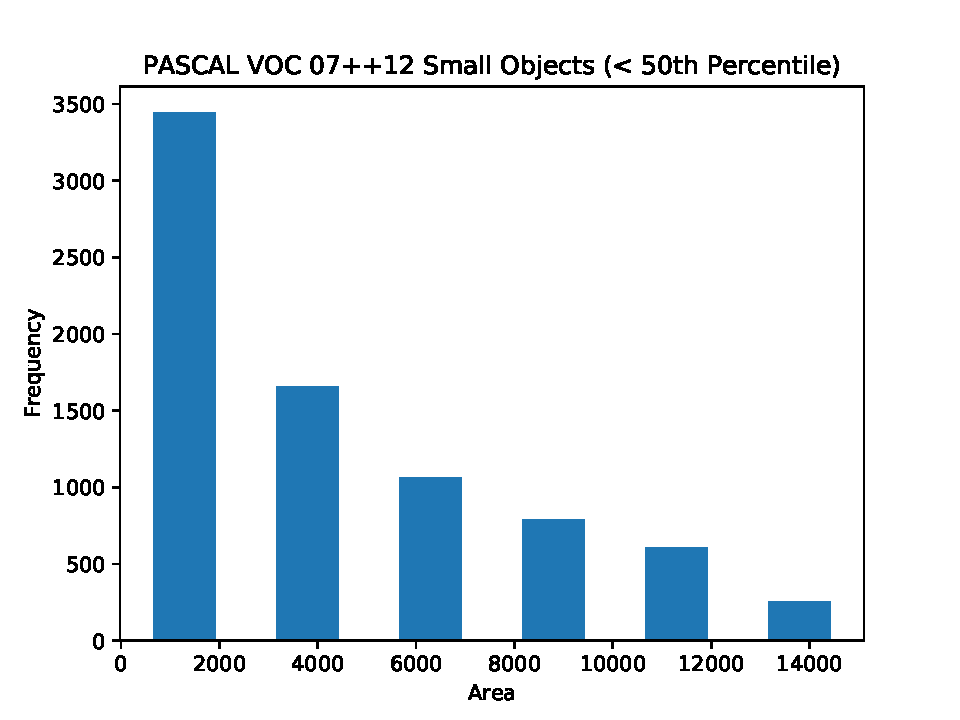
\includegraphics[width=\textwidth]{Figs/Implementation/testsmallhist.pdf}
        \caption{}\label{fig:smalltesthist}
    \end{subfigure}
    \begin{subfigure}[b]{0.45\textwidth}
        \center
        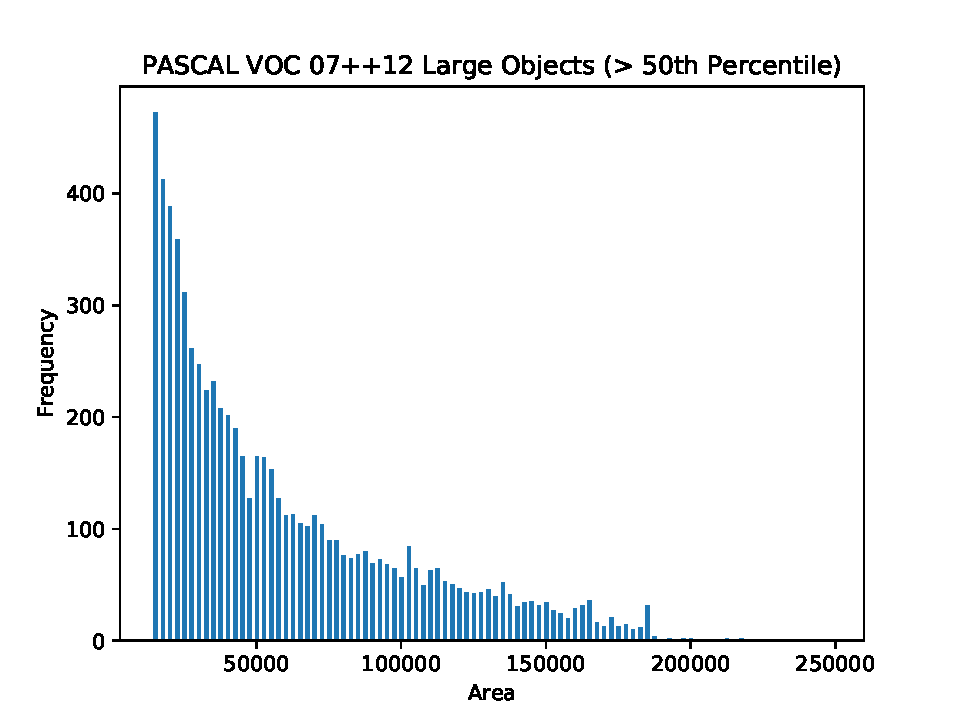
\includegraphics[width=\textwidth]{Figs/Implementation/testlargehist.pdf}
        \caption{}\label{fig:largetesthist}
    \end{subfigure}
    \caption{}
    \label{}
\end{figure} 

The results for the object detectors trained on the separate partitions of training data and a the baseline detector trained on all the data against the three sets of tests can be seen in \tableref{resresults}. The table shows that the detectors trained on the same relative size of data perform best. In the instance of 07Test$_{small}$, its counterpart 07++12$_{small}$ gives a result 04 0.34 \gls{map}. This is an improvement of 12\% in comparison to the model trained on all of the data (07++12) which has a \gls{map} of 22.16\%; a relative improvement of 35\%. The model trained on the data of larger objects, 07++12$_{larger}$, is very poor at detecting smaller objects scoring 3.08\%. In this case of 07Test$_{larger}$, the model trained on 07++12$_{larger}$ data is the best performing at 76.60\%. A similar improvement is \gls{map} is present in this instance in comparison to the model trained on all of the data. Overall there is an increase of 12.36\%, which is a relative improvement of 16\%. Finally, the best performing on all of the 07 test data is the model trained on 07++12.


\begin{table}[h]
\centering
\caption{Results}
\label{tab:resresults}
\begin{tabular}{|l|l|l|}
\hline
\textbf{Train Data}    & \textbf{Test Data}     & \textbf{mAP (\%)} \\ \hline
07++12$_{small}$ & 07Test$_{small}$  & \textbf{34.10}   \\ \hline
07++12$_{larger}$  & 07Test$_{small}$ & 3.08     \\ \hline
07++12   & 07Test$_{small}$           & 22.16    \\ \hline
07++12$_{small}$ & 07Test$_{larger}$  &  36.40   \\ \hline
07++12$_{larger}$ & 07Test$_{larger}$ &  \textbf{76.60}   \\ \hline
07++12 & 07Test$_{larger}$           &  64.34   \\ \hline
07++12$_{small}$       & 07   & 62.65    \\ \hline
07++12$_{larger}$       & 07  &  59.65   \\ \hline
07++12        & 07            &  \textbf{76.35}   \\ \hline 
\end{tabular}
\end{table}


\change[inline]{update following explanation}
Ensemble of above networks proved not to be possible due to Caffe network architecture. Once networks have been trained as an end-to-end method, the networks were not able to take object proposals as inputs. Solution instead to train the network in 5 stages. Much slower. Result on VOC2007: 79.59 vs end to end: 76.35 

While \tableref{resresults} shows that it is possible for a \gls{rfcn} network to be optimised to objects of a certain size, a more powerful approach is to combine the two networks in an ensemble during testing. Given a potential object, the ensemble should weight one of the networks outputs accordingly. A simple example in this case would be to weight one of the outputs by 100\%, if the potential object is below or above the threshold found in the training data. The results gathered in \tableref{resresults} are much more naive than this, simply splitting the testing data and only using one trained network at a time. Object proposals will needed to be known during inference to ensure that the outputs of the networks in an ensemble are performing classification in the same locations. On top of this, new networks will needed to be trained on subsets of smaller and larger data due to the internal architecture of \gls{caffe} networks. The networks in the ensemble will need to take object proposals as inputs, however, the above mentioned networks are trained based upon the end-to-end versions of the \gls{rfcn}. These do not take proposals as inputs but rather have an internal \gls{rpn}. Therefore, the new networks are trained using 4-step alternating training used in the original Faster R-CNN paper \cite{fasterrcnn}. 
\begin{comment}
    In this approach the overall network in trained in multiple steps rather than an end-to-end method. In step one a \gls{rpn} is trained to determine region proposals, the \gls{rpn} is initialised from a pre-trained ImageNet model and fine-tuned to the proposal task. Next a \gls{rfcn} is trained based upon the proposals found in the previous step. This network is also initialised with a pre-trained ImageNet model. In step three, another \gls{rpn} is trained but initialised using the \gls{rfcn} from step two. In this step the convolutional layers that are shared between the \gls{rfcn} and \gls{rpn} are fixed and only the layers unique to the \gls{rpn} are updated. In this final step, the shared layers between the two networks are again kept fixed and the layers unique to the \gls{rfcn} are updated. By training a model with this approach a testing image is able to run through the same steps as a \gls{rfcn} trained end-to-end, however, as the networks are split into different models it is also possible to use the stages of the method individually. Creating a solution for finding region proposals with an \gls{rpn} and having a \gls{rfcn} that can take the proposals as inputs. 
\end{comment}
\\\\
A potential shortcoming of using \gls{rpn} proposals as inputs to training a \gls{rfcn} rather than using ground truth bounding boxes is that a \gls{rpn} likely finds many more examples of objects that actually exist in an image. For a given image, an \gls{rpn} may find hundreds of potential objects despite an image only containing a couple of true positive examples. This can be solved by setting the proposals with the highest confidence as the ground truth examples and labelling the remaining proposals as the background class. This is a stark comparison to the end-to-end training approach as there are now many more training examples and a large skew towards the background class. Whereas the end-to-end approach does not train on any background examples. With this approach, the total number of training examples is increased from 80,116 to 9,979,345. The median of the almost 10 million proposals is 4,684 pixels, significantly smaller than the threshold of 19,205.5 determined using only ground truth boxes. This large increase in training examples and skew in data poses a question on how to split the \gls{rpn} proposals such that two networks can be trained towards small and large objects respectively. As mentioned earlier, a pre-requisite in creating subsets of data is that the multiple sets should be roughly equal in size in order for training to be conducted fairly. If the subsets were split by the median of the \gls{rpn} proposals (4,684) the two sets of data would have equal numbers of examples. However, upon inspection there seems to be a large skew in \gls{rpn} proposals to smaller objects as there are significantly more true positive examples in the subset of data containing larger objects. This can be seen in \tableref{splitrpn}, where despite there being an almost even split in data subsets there are significantly more ground truth annotations in the \gls{rpn}$_{larger}$ subset.

\begin{table}[h]
\centering
\caption{My caption}
\label{tab:splitrpn}
\begin{tabular}{|l|l|l|}
\hline
\textbf{Data} & \textbf{RPN$_{small}$} & \textbf{RPN$_{larger}$} \\ \hline
Ground Truth & 19,992    & 60,116     \\ 
Background   & 4,969,369 & 4,929,297  \\ \hline
Total        & 4,989,361 & 4,989,413  \\ \hline
\end{tabular}
\end{table}

Another option is to use the threshold of 19,205.5 found on only ground truth boxes used in the initial test. The data distribution based on this threshold can be seen in \tableref{splitgt}. In this instance there is significantly more data in the \gls{rpn}$_{larger}$ subset, however, the skew is solely due to the many more background examples. The ground truth annotations are shared equally with 40,058 in each.

\begin{table}[h]
\centering
\caption{My caption}
\label{tab:splitgt}
\begin{tabular}{|l|l|l|}
\hline
\textbf{Data} & \textbf{RPN$_{small}$} & \textbf{RPN$_{larger}$} \\ \hline
Ground Truth & 40,058    & 40,058     \\ 
Background   & 3,528,370 & 6,370,859  \\ \hline
Total        & 3,568,428 & 6,410,917  \\ \hline
\end{tabular}
\end{table}

As the overall goal of object detectors is to find objects within the $C$ classes, the decision was made to use the threshold of 19,205.5 to create the split in data. Despite there being significantly more background examples. 
\\\\
A baseline 4-step \gls{rfcn} with ResNet-101 model was trained on all the data (07++12).

\begin{table}[h]
\centering
\caption{My caption}
\label{my-label}
\begin{tabular}{|l|l|}
\hline
\textbf{Train Data} & \textbf{\gls{ap}}      \\ \hline
Small      & 46.74\% \\ \hline
Large      & 56.91\% \\ \hline
All        & 79.59\% \\ \hline
Fusion     & \textbf{81.81\%} \\ \hline
\end{tabular}
\end{table}


\begin{table}[h]
\centering
\caption{My caption}
\label{my-label}
\begin{tabular}{|l|l|}
\hline
\textbf{Train Data} & \textbf{\gls{ap}}      \\ \hline
Small      & \textbf{55.00\%} \\ \hline
Large      & 10.86\% \\ \hline
All        & 43.80\% \\ \hline
\end{tabular}
\end{table}


\begin{table}[h]
\centering
\caption{My caption}
\label{my-label}
\begin{tabular}{|l|l|}
\hline
\textbf{Train Data} & \textbf{\gls{ap}}      \\ \hline
Small      & 21.28\% \\ \hline
Large      & \textbf{80.10\%} \\ \hline
All        & 75.14\% \\ \hline
\end{tabular}
\end{table}








